% A simple template for Beamer presentations in LaTeX
% 
% To produce pdf run:
%   $ pdflatex beamer.tex 
%

\documentclass{beamer}
\usetheme{Singapore}

\hypersetup{colorlinks=true}

% Graphics examples
%\centerline{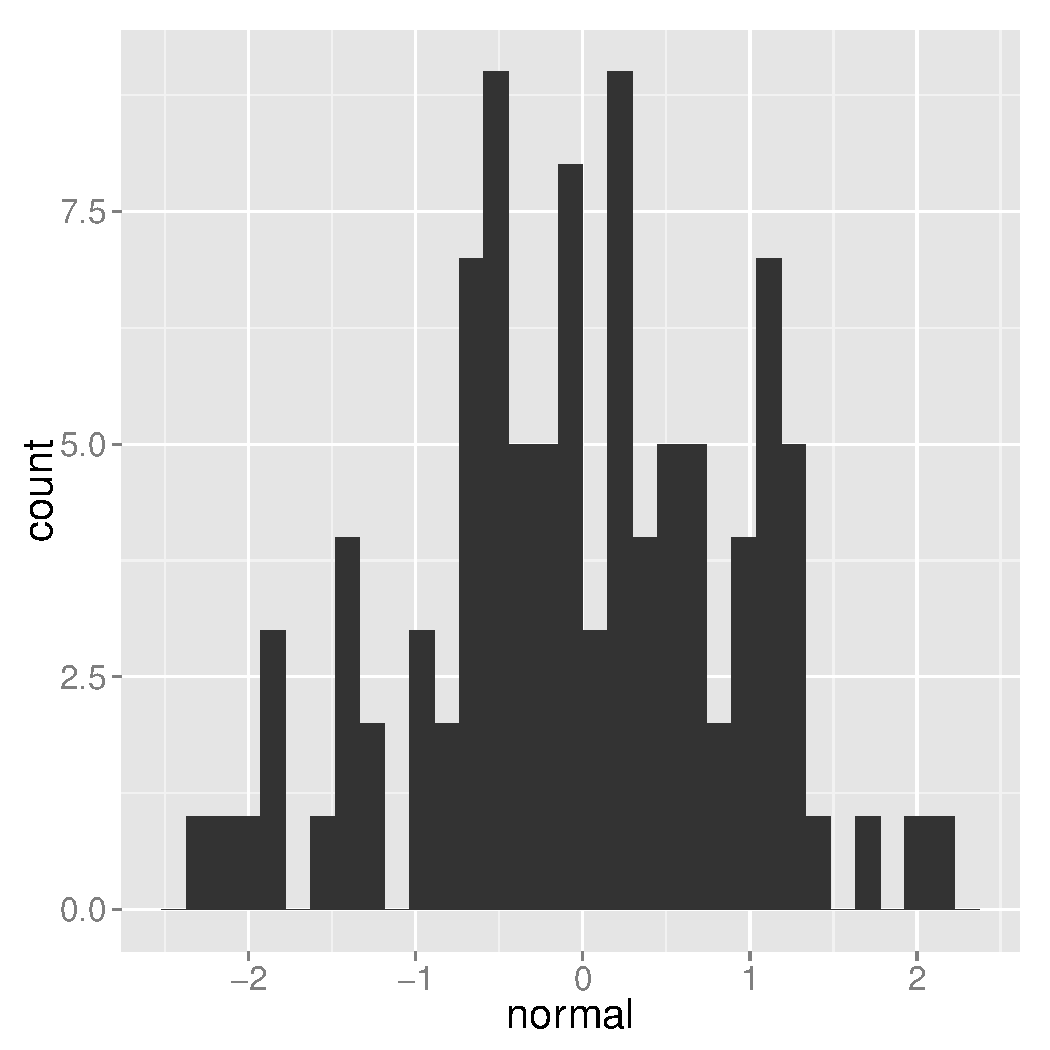
\includegraphics[height=2.5in]{figs/normal.pdf}}
%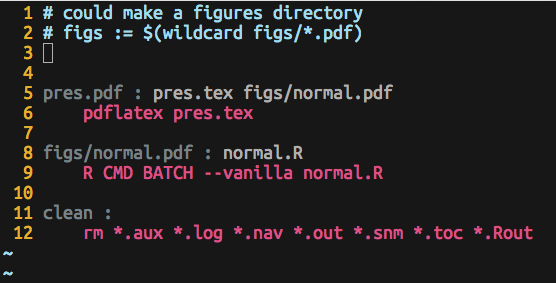
\includegraphics[width=4in]{figs/makefile.png}

%%%%%%%%%%%%%%%%%%%%%%%%%%%%%%%%%%%%%%%%%%%%%%%%%%%%%%%%%%%%

\begin{document}

\title[Python] % (optional, only for long titles)
{Data Mining with Python}
\subtitle{Most of the work is in preparing the data}
\author{Clark Fitzgerald - @clarkfitzg}
\institute{UC Davis - Statistics}
\date{Winter 2014} % (optional)
\subject{Statistics}

\frame{\titlepage}


%%%%%%%%%%%%%%%%%%%%%%%%%%%%%%%%%%%%%%%%%%%%%%%%%%%%%%%%%%%%
\begin{frame}


\frametitle{Statisticians \emph{love} data visualizations}

Here's some random math thing.
\[
    f(x, n) = \sum_{i=1}^n x i^2 + 23x + \pi
\]
More text after.

    \begin{block}{Summary}
    Programming is super fun.
    \end{block}


\end{frame}
%%%%%%%%%%%%%%%%%%%%%%%%%%%%%%%%%%%%%%%%%%%%%%%%%%%%%%%%%%%%
\begin{frame}


\frametitle{This is the second slide}
Here is where I would write a bunch of text. Visit the course website\footnote{\url{https://github.com/nick-ulle/2015-python-course}}

\begin{itemize}
\item Bullet 1
\item Bullet 2
\end{itemize}


\end{frame}
%%%%%%%%%%%%%%%%%%%%%%%%%%%%%%%%%%%%%%%%%%%%%%%%%%%%%%%%%%%%
\begin{frame}[fragile]


\frametitle{Code block}

Need to use `fragile` for a code block.

\begin{verbatim}

# Everything in the `figs` directory
figs := $(wildcard figs/*)

pres.pdf : pres.tex $(figs)
    pdflatex pres.tex

\end{verbatim}


\end{frame}
%%%%%%%%%%%%%%%%%%%%%%%%%%%%%%%%%%%%%%%%%%%%%%%%%%%%%%%%%%%%

\end{document}
